\section{Ciepły start}\label{chapter:results_warm_start}

\begin{figure}[h]
    \centering
    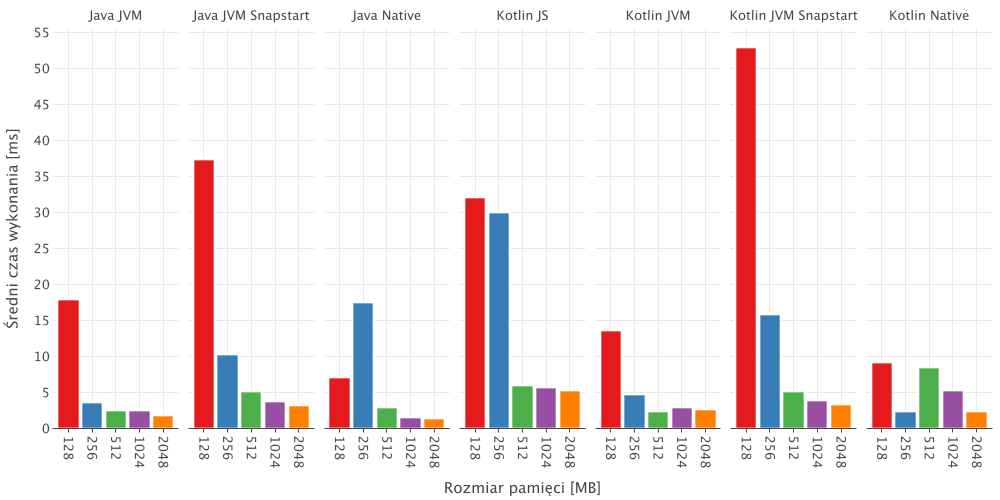
\includegraphics[width=0.95\textwidth]{charts/results/avg-warm-start.png}
    \caption{Średni czas wykonywania funkcji (ciepły start) w zależności od rozmiaru pamięci [źródło: opracowanie własne]}
    \label{fig:avg_warm_start}
\end{figure}

% --- Row 1: 256 MB and 1024 MB charts ---
\begin{figure}[htbp]
    \centering % Center the minipages on the line
    \begin{minipage}[t]{0.48\textwidth} % [t] for top alignment
        \centering % Center content within this minipage
        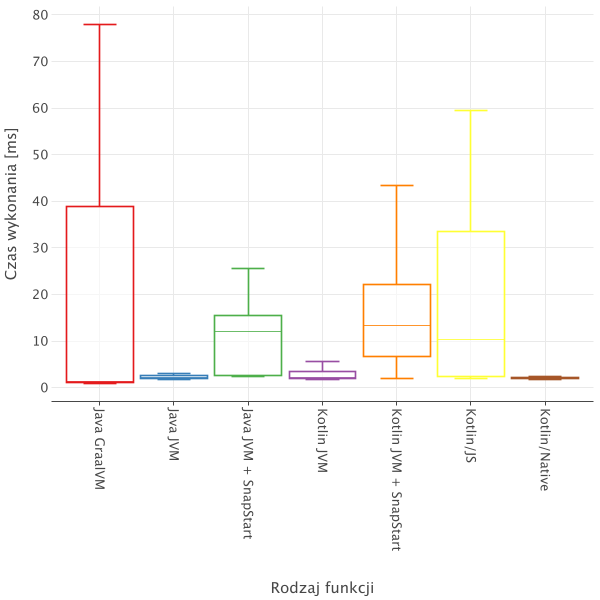
\includegraphics[width=\linewidth]{charts/results/warm-start-boxplot-256.png}
        \captionof{figure}{Czas wykonania funkcji (ciepły start, 256 MB) [źródło: opracowanie własne]}
        \label{fig:warm_start_128} % Unique label for this figure
    \end{minipage}% <--- % is important
    \hfill % Space between minipages
    \begin{minipage}[t]{0.48\textwidth}
        \centering
        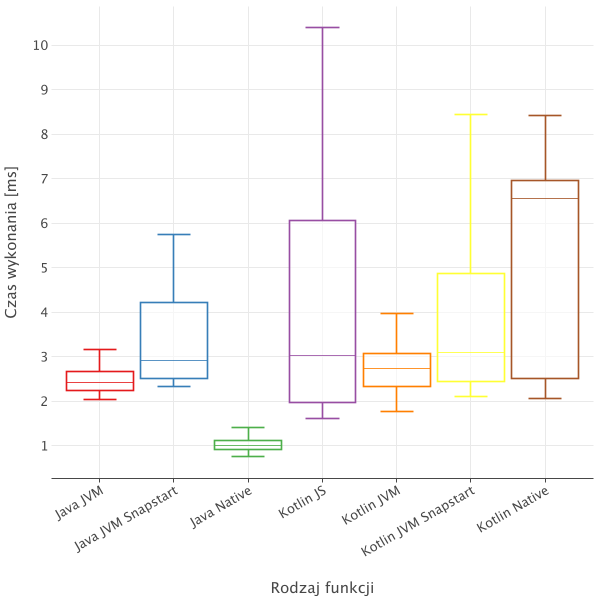
\includegraphics[width=\linewidth]{charts/results/warm-start-boxplot-1024.png}
        \captionof{figure}{Czas wykonania funkcji (ciepły start, 1024 MB) [źródło: opracowanie własne]}
        \label{fig:warm_start_256} % Unique label
    \end{minipage}
    % No overall \caption for this outer figure environment, as it's just for layout.
\end{figure}
